\section{What the explicit property mode contributes (E9)}
\label{sec:e9}

\subsection{Frozen dimensionality comparison}
E8 showed that the original rigid fourth-order model was worse than independent third-order property models in physical-unit RMSE. E9 retains that result and asks the narrower question for which TBMD was introduced: whether an explicit property axis improves relative field recovery or spatial structure when capacity, measurements and recovery are matched. Before computing any new E9 outer metric, we froze H1--H5, the anomaly-relative error and mask-aware anomaly SSIM in Section~\ref{sec:metrics}, two capacity controls, five fourth-order architectures, sensor budgets, a three-fold inner selection loss and the fold-consistency rule. The complete inner registry contains \ENineRepresentationRows{} representation and \ENineSparseRows{} sparse-recovery rows; all planned fits succeeded. Each of the \ENineOuterRows{} outer records was then generated in one pass over the frozen fold configurations.

Training-only dependence diagnostics support partial sharing: a common temporal direction coexists with weakly aligned property-specific spatial directions (Supplementary Section~S8). Full property rank adds no property compression.

\subsection{Current joint model versus optimized partial coupling}
The corrected metrics do not rescue the current rigid model: it meets the E9 advantage rule in only \ENineCurrentAdvantages{} of \ENineHeadlineComparisons{} headline comparisons. Its shared coefficients remain a severe restriction, especially for saturation. By contrast, train-only selection chooses 4D-B---shared spatial factors with separate property coefficients---in \ENineSharedHeadSelections{} of \ENineSparseSelections{} sparse fold/budget comparisons and in every full-observation comparison. Removing independent heads (4D-A/C) recreates the pressure--saturation compromise; property rank one is never selected for 4D-A.

With full observation and equal total capacity, optimized 4D lowers pressure anomaly error from \ENineFullThreeErrorP{} to \ENineFullFourErrorP{} and raises pressure anomaly SSIM from \ENineFullThreeSsimP{} to \ENineFullFourSsimP. Saturation error instead changes from \ENineFullThreeErrorSo{} to \ENineFullFourErrorSo, without a fold-consistent structural gain. The fourth-order representation therefore supplies a modest pressure and storage benefit (\ENineFullFourStorage{} versus \ENineFullThreeStorage{} stored floats), not universally better approximation.

Sparse observations produce the scientifically relevant gain. With 30 common grid channels, pressure/saturation anomaly error falls from \ENineGridThirtyThreeErrorP/\ENineGridThirtyThreeErrorSo{} to \ENineGridThirtyFourErrorP/\ENineGridThirtyFourErrorSo, while anomaly SSIM rises from \ENineGridThirtyThreeSsimP/\ENineGridThirtyThreeSsimSo{} to \ENineGridThirtyFourSsimP/\ENineGridThirtyFourSsimSo. Both properties and both endpoints meet the fold-consistency rule in both capacity controls. The same four-way advantage occurs at five existing wells. At 300 grid channels, the equal-total comparison remains favourable on all four endpoints (\ENineGridThreeHundredThreeErrorP/\ENineGridThreeHundredThreeErrorSo{} versus \ENineGridThreeHundredFourErrorP/\ENineGridThreeHundredFourErrorSo; SSIM \ENineGridThreeHundredThreeSsimP/\ENineGridThreeHundredThreeSsimSo{} versus \ENineGridThreeHundredFourSsimP/\ENineGridThreeHundredFourSsimSo). Intermediate well budgets and equal-per-property saturation error are more mixed; complete fold values and paired differences are retained in the canonical output.

% Generated by e9_analyze.py; do not edit.
\begin{table*}[htbp]\centering\small
\caption{E9 equal-total-capacity anomaly reconstruction: 32 coefficients per model, identical observations and common inner-selected solver. $E'$ is anomaly-relative error (lower is better); SSIM$'$ is mask-aware anomaly structural similarity (higher is better). Budget counts scalar channels for grid sensing and two-property wells for well sensing. Values are mean $\pm$ sample standard deviation over ten outer scenarios. 3D and 4D denote the independently train-selected models.}
\label{tab:e9_headline}
\setlength{\tabcolsep}{3pt}
\begin{adjustbox}{max width=\textwidth}
\begin{tabular}{lrlrrrr}\toprule
Geometry & Budget & Model & $E^\prime_p$ & $E^\prime_{S_o}$ & SSIM$^\prime_p$ & SSIM$^\prime_{S_o}$ \\ \midrule
grid & 30 & 3D & 1.167 $\pm$ 0.619 & 0.844 $\pm$ 0.287 & 0.406 $\pm$ 0.392 & 0.856 $\pm$ 0.034 \\
grid & 30 & 4D & 0.350 $\pm$ 0.162 & 0.465 $\pm$ 0.135 & 0.770 $\pm$ 0.254 & 0.932 $\pm$ 0.019 \\
grid & 300 & 3D & 0.148 $\pm$ 0.071 & 0.375 $\pm$ 0.114 & 0.941 $\pm$ 0.036 & 0.927 $\pm$ 0.026 \\
grid & 300 & 4D & 0.096 $\pm$ 0.039 & 0.348 $\pm$ 0.088 & 0.967 $\pm$ 0.021 & 0.948 $\pm$ 0.018 \\
wells & 5 & 3D & 0.498 $\pm$ 0.265 & 2.071 $\pm$ 0.378 & 0.818 $\pm$ 0.145 & 0.762 $\pm$ 0.011 \\
wells & 5 & 4D & 0.421 $\pm$ 0.287 & 0.950 $\pm$ 0.174 & 0.922 $\pm$ 0.039 & 0.866 $\pm$ 0.020 \\
wells & 15 & 3D & 0.212 $\pm$ 0.120 & 1.059 $\pm$ 0.242 & 0.939 $\pm$ 0.035 & 0.850 $\pm$ 0.029 \\
wells & 15 & 4D & 0.207 $\pm$ 0.092 & 0.890 $\pm$ 0.078 & 0.968 $\pm$ 0.016 & 0.868 $\pm$ 0.023 \\
wells & 30 & 3D & 0.191 $\pm$ 0.120 & 0.733 $\pm$ 0.154 & 0.920 $\pm$ 0.062 & 0.882 $\pm$ 0.032 \\
wells & 30 & 4D & 0.121 $\pm$ 0.092 & 0.722 $\pm$ 0.274 & 0.965 $\pm$ 0.035 & 0.894 $\pm$ 0.042 \\
\bottomrule\end{tabular}
\end{adjustbox}
\end{table*}


\begin{figure*}[htbp]
\centering
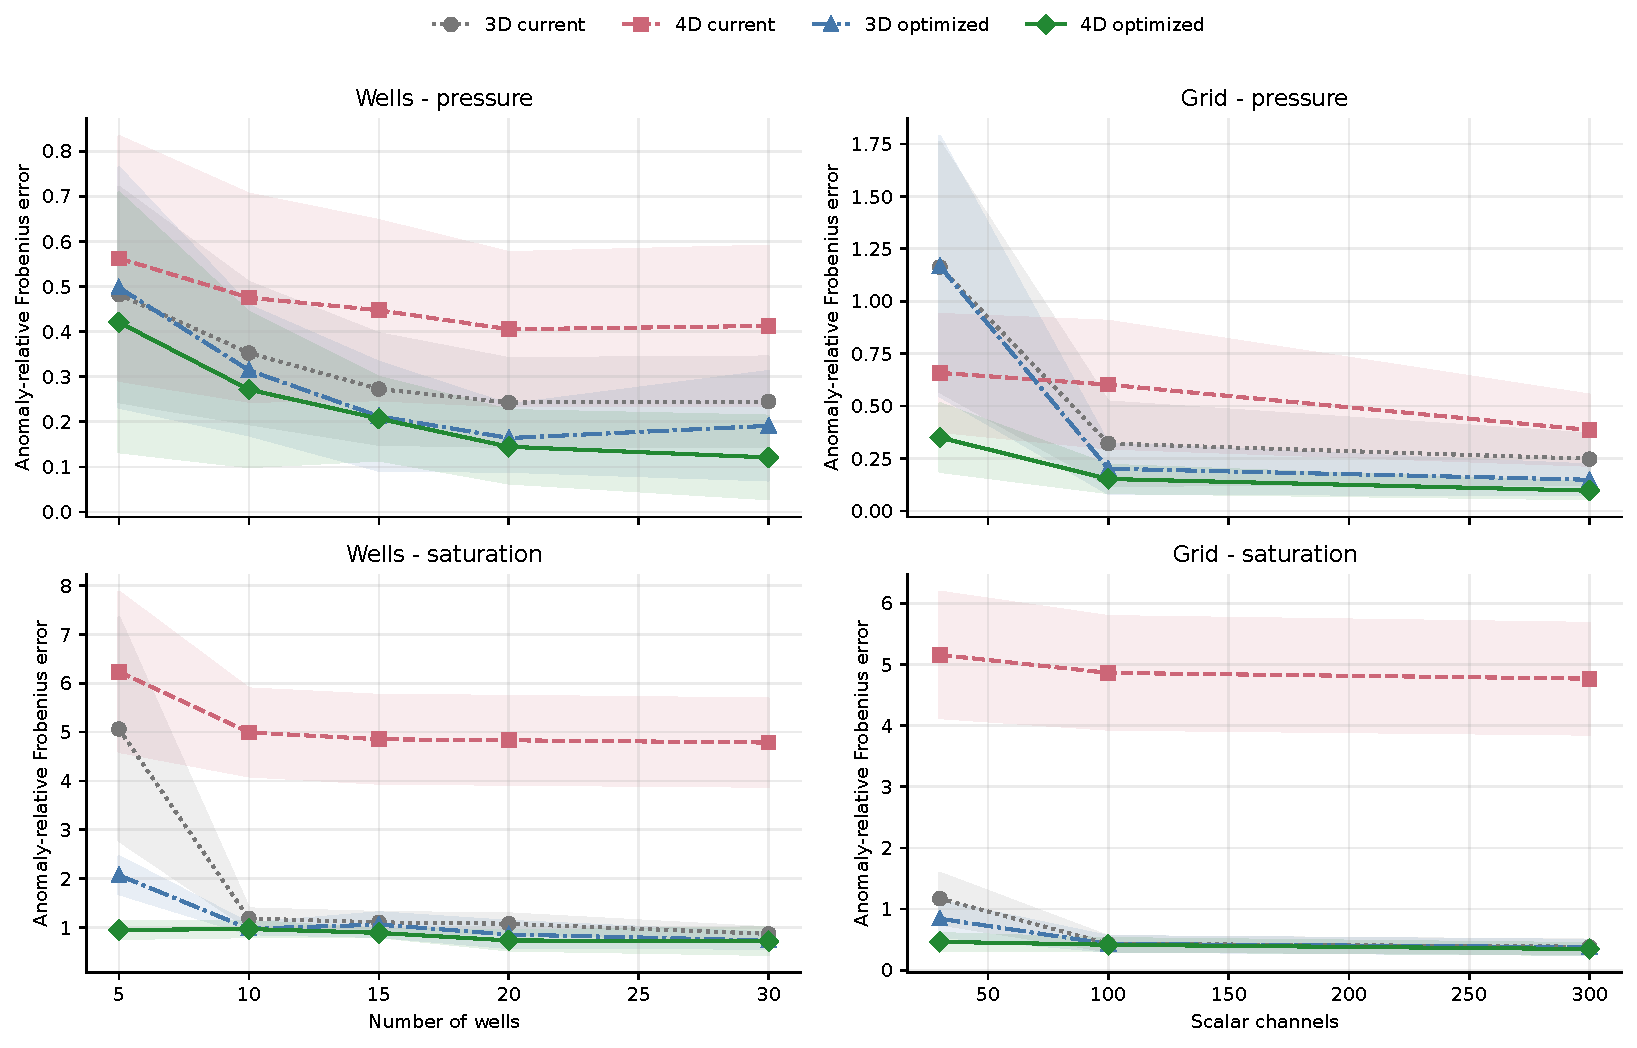
\includegraphics[width=\textwidth]{../../../studies/brugge_sparse_sensing/figures/fig15_e9_reconstruction_error.pdf}
\caption{E9 anomaly-relative reconstruction error against the common sensor budget under equal-total capacity. Curves show the current independent 3D/current rigid 4D pair and their train-selected counterparts. Every point is a mean over ten untouched outer folds; shaded bands show one sample standard deviation. Lower is better.}
\label{fig:e9_error}
\end{figure*}

\begin{figure*}[htbp]
\centering
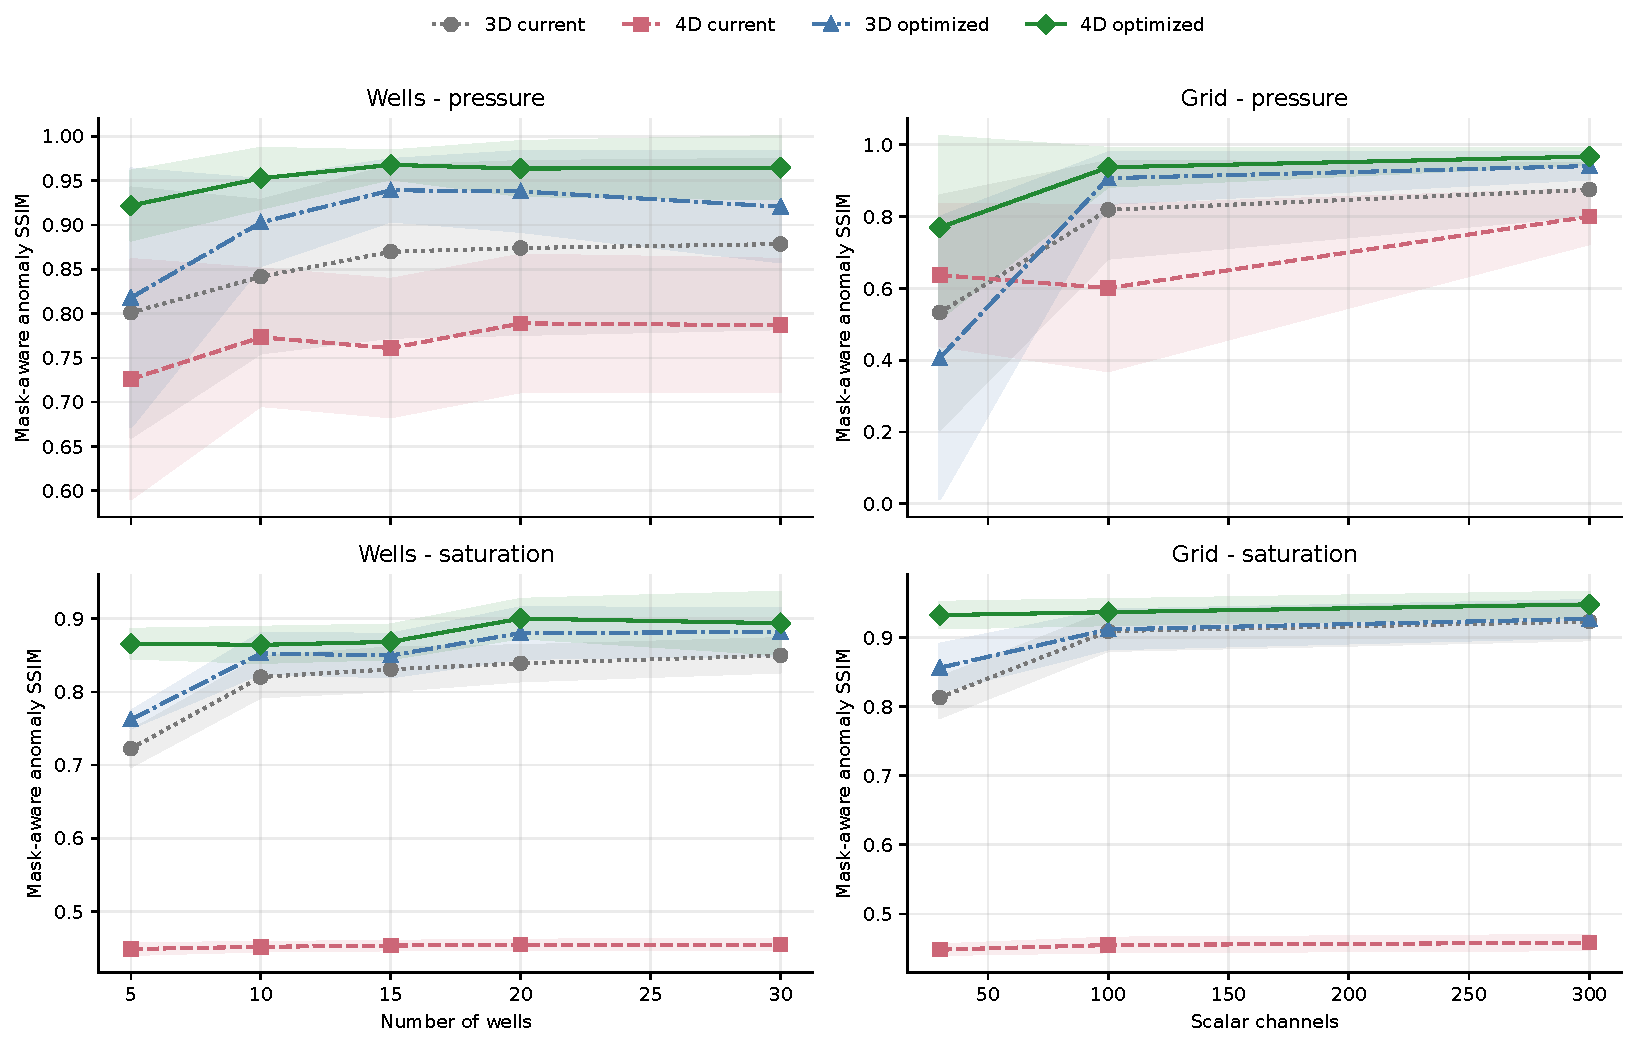
\includegraphics[width=\textwidth]{../../../studies/brugge_sparse_sensing/figures/fig16_e9_ssim.pdf}
\caption{Mask-aware anomaly SSIM for the same E9 comparisons. Panels show pressure (top) and oil saturation (bottom), versus well (left) or scalar grid-channel (right) budget; mean and one sample standard deviation across ten outer folds, equal-total capacity. Inactive background is excluded. Higher is better.}
\label{fig:e9_ssim}
\end{figure*}

\subsection{Metric concordance and structural fidelity}
RMSE, anomaly-relative error and anomaly SSIM rank the optimized pair identically in all but \ENineRankingDifferences{} of \ENineRankingRegimes{} property/regime comparisons. The exceptions bound the claim. At 15 wells under equal-total capacity, 3D has lower mean pressure RMSE (\ENineWellFifteenThreeRmseP{} versus \ENineWellFifteenFourRmseP), whereas 4D has lower anomaly error (\ENineWellFifteenThreeErrorP{} versus \ENineWellFifteenFourErrorP) and higher anomaly SSIM (\ENineWellFifteenThreeSsimP{} versus \ENineWellFifteenFourSsimP); only the SSIM gain satisfies the fold rule. At 300 grid channels under equal-per-property capacity, saturation pointwise metrics favour 3D but structural similarity favours 4D. These are structural-fidelity results, not restated accuracy wins.

Figure~\ref{fig:e9_maps} was fixed to scenario~1, report step 132 and 15 configured wells before outer evaluation. In that snapshot, 4D-B has higher pressure pointwise error but higher pressure anomaly SSIM, while it improves both saturation endpoints. The maps make the distinction between local structural preservation and absolute error visible.

\begin{figure*}[htbp]
\centering
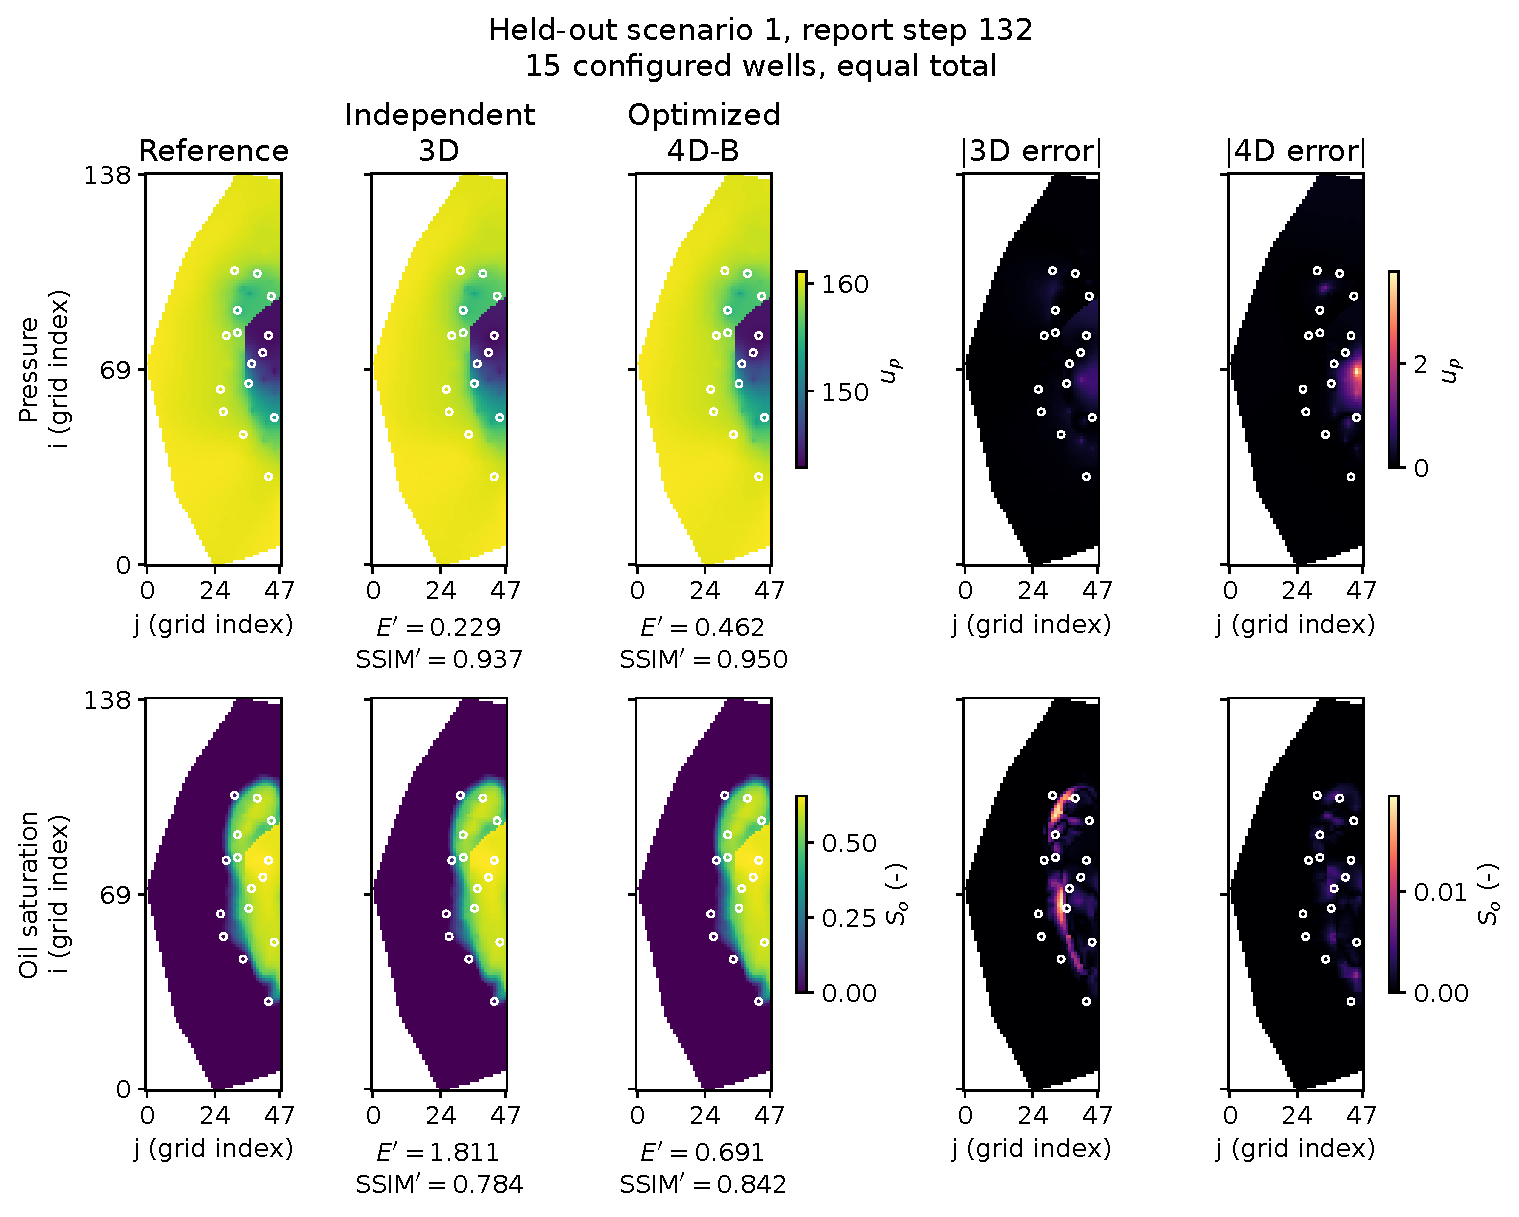
\includegraphics[width=\textwidth]{../../../studies/brugge_sparse_sensing/figures/fig19_e9_reconstruction_maps.pdf}
\caption{Fixed E9 reconstruction example. Columns show reference, independent 3D, train-selected shared-factor 4D-B, and matched absolute-error maps for pressure (top) and oil saturation (bottom). Axes are grid indices (no physical distances are available); white circles mark the 15 observed wells and inactive cells are blank. Pressure is in $u_p$ and saturation is dimensionless. All state panels share limits within each property, as do the paired absolute-error panels; panel annotations are snapshot-specific anomaly error and mask-aware anomaly SSIM.}
\label{fig:e9_maps}
\end{figure*}

The E9 advantage is conditional on coupling architecture, observation budget and metric. Shared-factor estimation can help sparse recovery; rigid coefficients, property rank one and full-state saturation approximation are not supported as general improvements.
